\chapter{Results}
\label{chap:results}

\section{Interface}
\todo{write something about performance. when does mesh become too heavy for VR rendering}
\todo{mention user fatigue, both with respect to controller and VR in general}
As mentioned in the previous chapter, SketchMeshVR does not make use of any menus and instead solely relies on different combinations of button presses to differentiate between the multiple available modeling actions. This does require more effort from the user in order to keep track of the selected editing modes, but at the same time keeps the interface cleaner. In order to guide the user when drawing strokes, SketchMeshVR provides visual feedback on the positions that will be used to create a stroke. In case of the drawing and curve deformation modes this means that the user sees the position controller and in case of all other modes the user will see the position controller plus a ray shooting from it (the ray ends at any intersections it has with the scene). Figures~\ref{fig:interface}(a) and (b) show what this looks like.

\begin{figure}[!h]
    \centering
    \setlength{\tabcolsep}{0.0130\linewidth}
    \begin{tabular}{@{}cc@{}}
    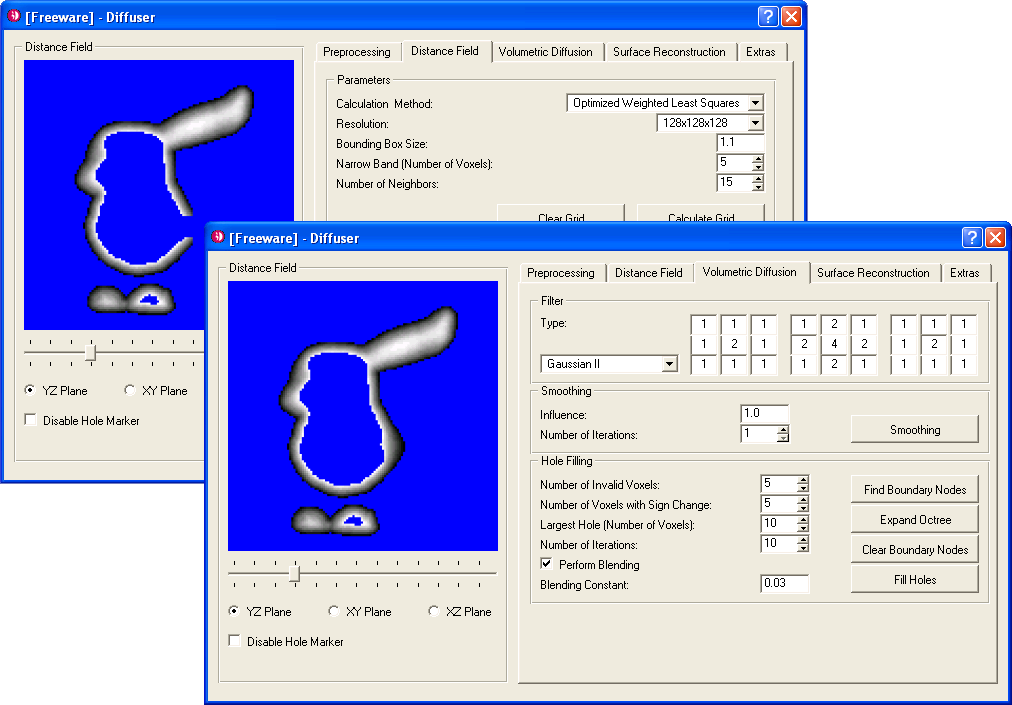
\includegraphics[width=0.3\linewidth]{figures/voldiff_ui}&
  	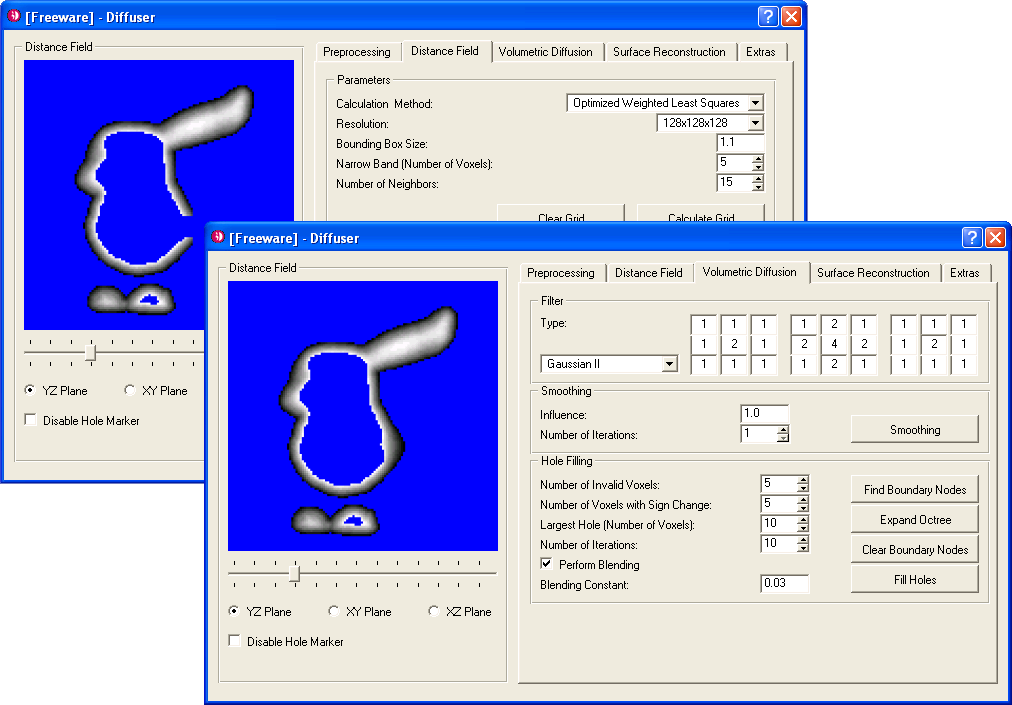
\includegraphics[width=0.3\linewidth]{figures/voldiff_ui}\\
    (a)&(b)\\
    \end{tabular}
    \caption[SketchMeshVR interface]{SketchMeshVR interface.
    	  \textup{(a)} Controller reference point that is displayed in drawing and deformation mode.
			  \textup{(b)} Controller and ray reference that are displayed in all other editing modes. 
      \label{fig:interface}}
\end{figure}
 
\section{User review}

\textcolor{red}{TODO:}
\begin{itemize}
\item mention test users' prior experience with 3D modeling and VR
\item explain test setup: asking users to recreate an example model both in VR \& non-VR version of program
\item summarize any comments they have on the test/experience
\item what did they think of ease of learning/modeling?
\item Is there a difference in efficiency between modeling in VR or non-VR?
\item show side-by-side comparisons of example model and user recreations
\end{itemize}


\todo{write what users experienced and show some created meshes}
Our program has been tested by several users that had none to little prior experience with 3D modelling and also had none to little experience with VR. The test users were requested to first model something \todo{probably specify what} using SketchMeshVR and then to recreate that model in the non-VR version of the software. Users reported that although it took some initial effort to get acquainted with the controls, it was very easy to learn how to use SketchMeshVR. They also reported that the immersive nature of VR made the interaction with the created mesh much more impressive compared to the non-VR SketchMesh. Although the users had experience with creating the given model when they modelled it in non-VR, it took them longer \todo{include: X seconds longer because non-VR took Y seconds while modelling a similar model in VR only took Z seconds) }to recreate the model than when using SketchMeshVR. Figures~\ref{fig:recreate_teddy} and~\ref{fig:recreate_dolphin} show side-by-side comparisons of the example models that were given to the test users, and the models that they created in both the non-VR and VR versions of our software. As you can see, the user successfully managed to recreate the example models that were provided to them. It is also clear that recreating the model in VR was significantly faster than in non-VR. \todo{check that this is actually true}


\begin{figure}[!h]
    \centering
    \setlength{\tabcolsep}{0.0130\linewidth}
    \begin{tabular}{@{}ccc@{}}
    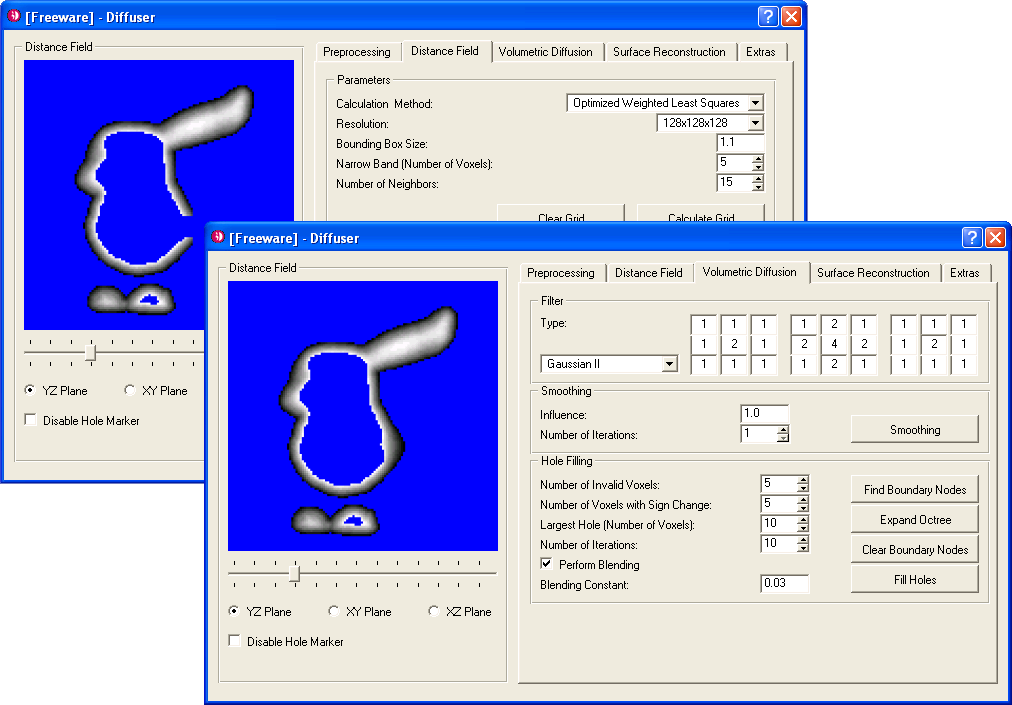
\includegraphics[width=0.3\linewidth]{figures/voldiff_ui}&
  	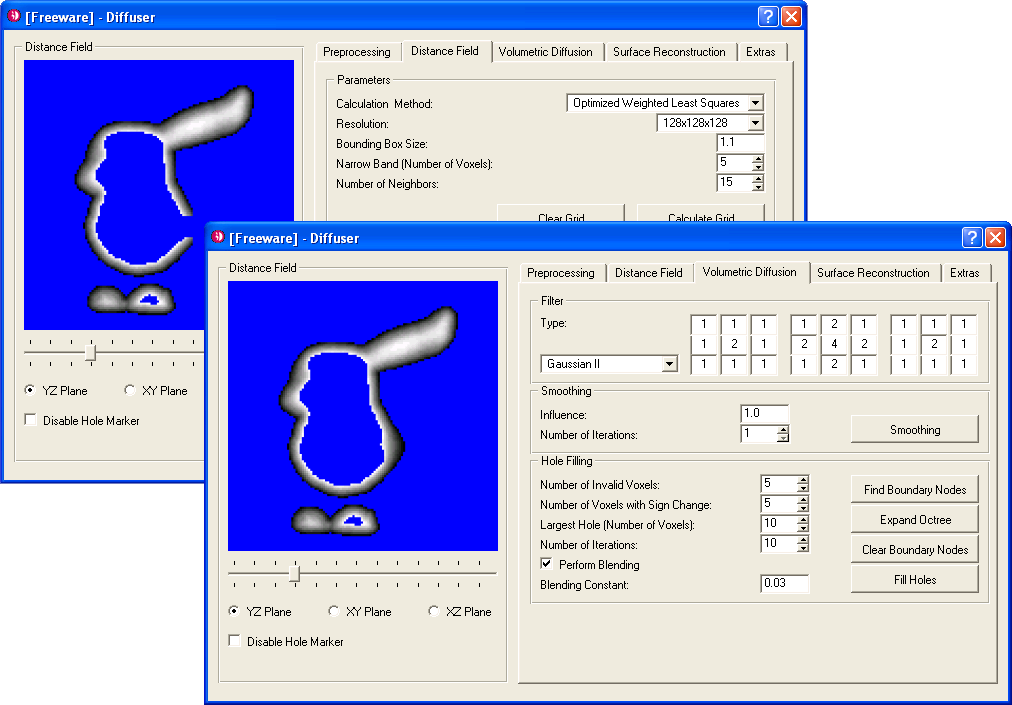
\includegraphics[width=0.3\linewidth]{figures/voldiff_ui}&
  	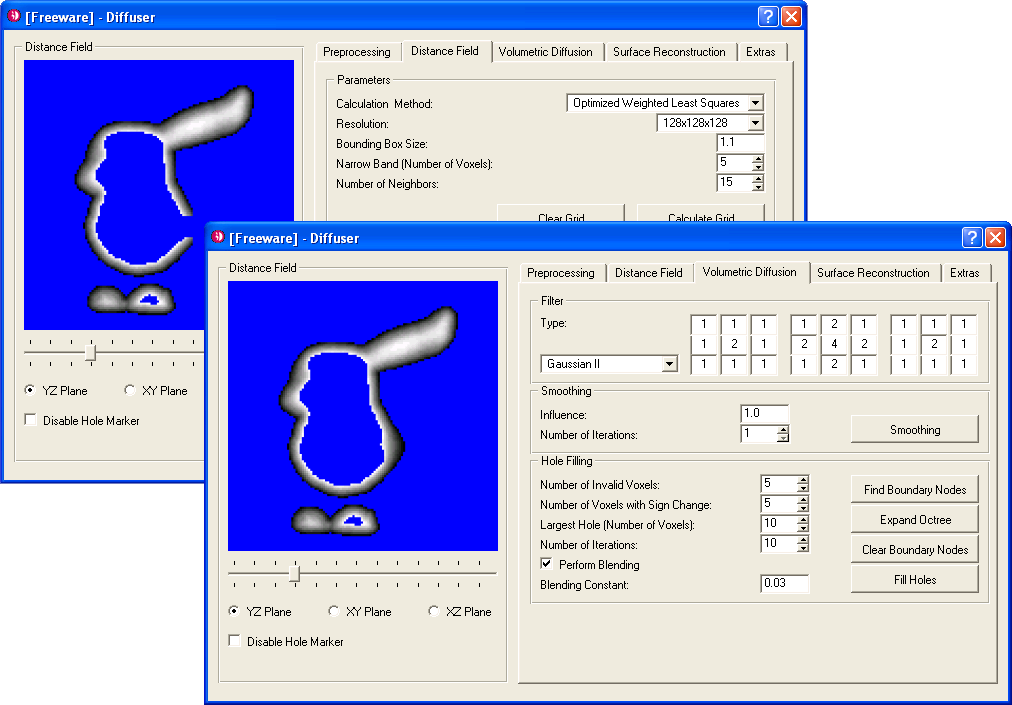
\includegraphics[width=0.3\linewidth]{figures/voldiff_ui}\\

    (a)&(b)&(c)\\
    \end{tabular}
    \caption[SketchMeshVR teddy model]{SketchMeshVR recreating models.
    	  \textup{(a)} Example simplified mesh of a teddy bear.
	  \textup{(b)} Resulting recreated model made in VR  (took X seconds to complete).
	  \textup{(c)} Resulting recreated model made in non-VR (took Y seconds to complete).
      \label{fig:recreate_teddy}}
\end{figure}
\todo{Fill in taken seconds in caption}


\begin{figure}[!h]
    \centering
    \setlength{\tabcolsep}{0.0130\linewidth}
    \begin{tabular}{@{}ccc@{}}
    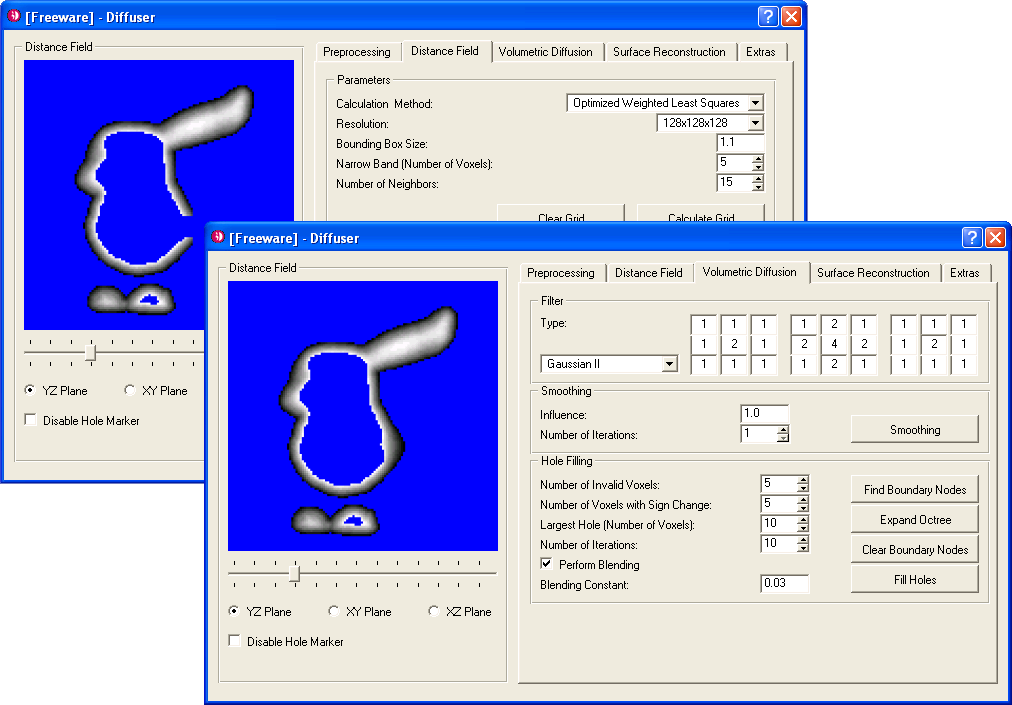
\includegraphics[width=0.3\linewidth]{figures/voldiff_ui}&
  	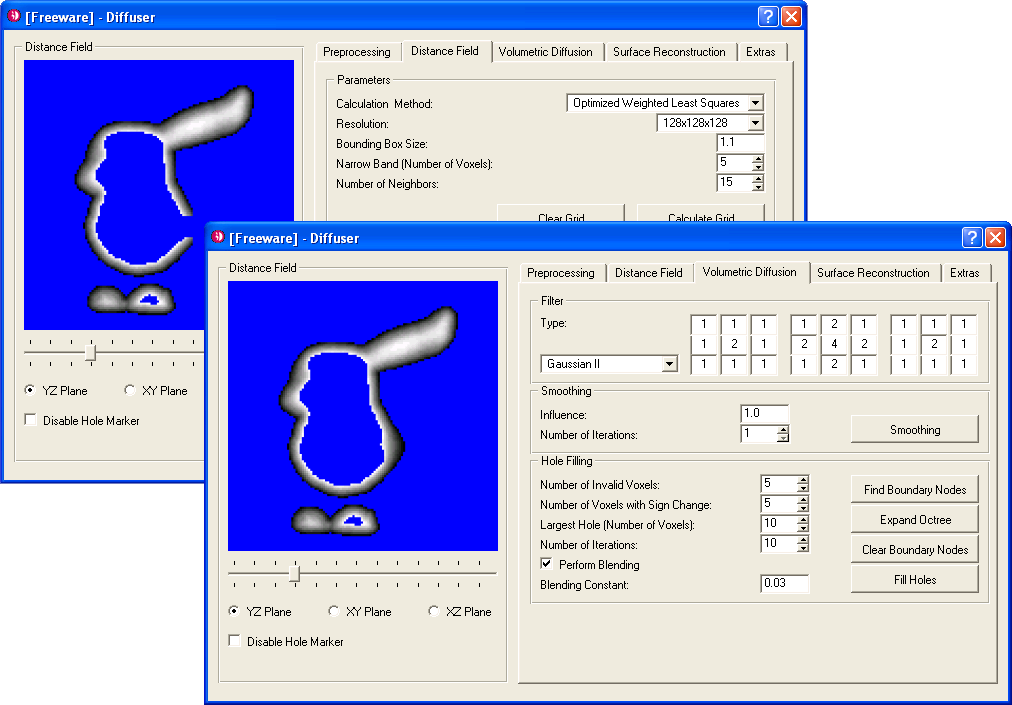
\includegraphics[width=0.3\linewidth]{figures/voldiff_ui}&
  	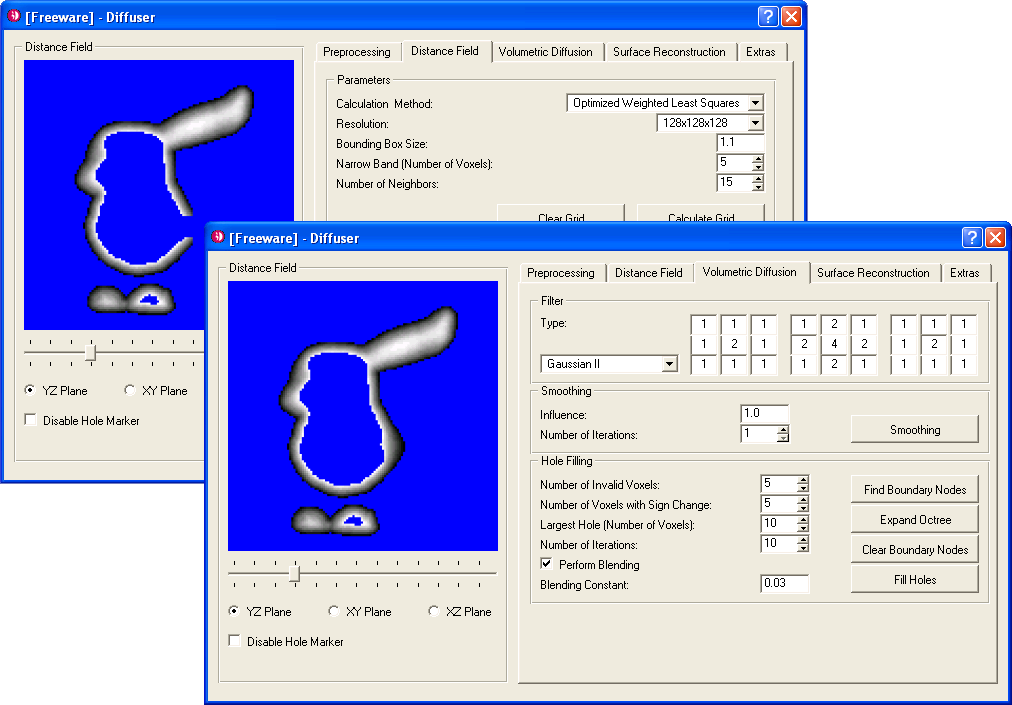
\includegraphics[width=0.3\linewidth]{figures/voldiff_ui}\\

    (a)&(b)&(c)\\
    \end{tabular}
    \caption[SketchMeshVR dolphin model]{SketchMeshVR recreating models.
    	  \textup{(a)} Example simplified mesh of a dolphin.
	  \textup{(b)} Resulting recreated model made in VR (took X seconds to complete).
	  \textup{(c)} Resulting recreated model made in non-VR (took Y seconds to complete).
      \label{fig:recreate_dolphin}}
\end{figure}
\todo{Fill in taken seconds in caption}


Also the users reported that they found the modelling to be considerably more effortless in VR, as it requires less intermediate navigation of the mesh between modelling steps (for example before drawing the extrusion silhouette or making a diagonal cut there is no need to rotate the mesh in VR). 
Additionally users noted that the possibility to define strokes in an additional dimension provides added artistic freedom, for example when defining the extrusion silhouette the user can now draw a S-shaped curve and choose where it will be positioned inside the extrusion base. 
